\begin{figure}[htp]
	\centering
	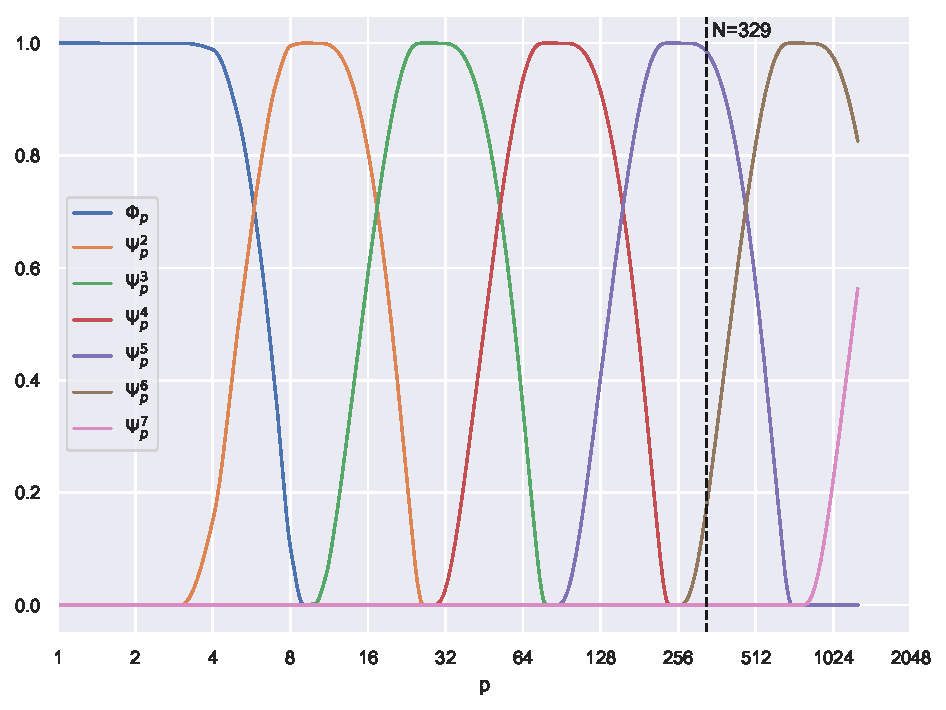
\includegraphics[width=\textwidth]{homer_slepian_tiling_b1275.pdf}
	\caption{
		The tiling of the Slepian line with parameters \(\lambda=3\) and \(J_{0}=2\) with \(\num{1275}\) basis functions.
		The black dashed line marks the Shannon number for the Homer head region \(N=329\).
		It is clear that the scaling function and the first five wavelets are non-zero as the coefficients are within the Shannon number.
	}\label{fig:chapter4_tiling}
\end{figure}
